\lab{Git and Bitbucket (BYU ACME Edition)}{BYU ACME Git}
\label{appendix:git2}
\objective{
Computer code is delicate.
A rogue or clumsy programmer can easily damage a program with a simple spelling error.
Maintaining a working product is therefore a serious endeavor in software development, requiring checks, collaboration, and careful coordination.
\emph{Git} is a version control system that facilitates code development involving multiple contributors.
It is commonly used to manage large projects, especially open-source projects, but it can also be used for personal code storage and management.
In this appendix we introduce Git and Bitbucket, a web-based hosting service for Git.
This tutorial does not require any previous programming experience.
}

% TODO: Set up a BYU ACME TA account on Bitbucket with two repositories: one for the students to import, and one for the TA's to import.

\section*{Overview} % =========================================================

The main idea behind Git is that the master copy (the official version) of a program's code is kept in the cloud in a \emph{repository}.
All certified contributors can \emph{clone} the repository onto their machine so that they can make changes to the code.
All changes are then submitted to the cloud, reviewed, and approved before the changes are \emph{merged} into the master copy.

If two contributors make changes to the same piece of code, it may create a \emph{merge conflict}, which must be resolved before any changes can be merged in.
For small repositories with few collaborators, merge conflicts are very rarely a problem.
The main issue then becomes understanding how to communicate edits between a local copy and the master copy in the cloud.

\subsection*{Installation} % --------------------------------------------------

Download the appropriate installer at \url{http://git-scm.com/downloads}.
Git is underlying software that will be accessed through the command line, so the installation will not create a new visible application.
On Windows machines, however, it will also download a terminal-like interface just for Git called \emph{git bash}.
Most Linux and Macintosh machines come with Git pre-installed.

\subsection*{Creating a New Repository} % -------------------------------------

A repository is the place where all of the code for an associated project resides.
Many different companies have websites for hosting Git repositories.
We will use Atlassian Inc.'s \href{https://bitbucket.org/}{\emph{Bitbucket}} because it is free to set up a limited number of private repositories.
Other popular repository hosts include \href{https://github.com/}{Github}, \href{https://gitlab.com/}{Gitlab}, and others.

There are two ways to set up a new repository: by importing an existing repository, or by starting from scratch.
We have a template repository for you to import, but most Git hosts present easy instructions for creating and setting up an empty repository.
For now, complete these steps to import the template repository:

\begin{enumerate}
\item Make an account at \url{https://bitbucket.org}.
Choose a user name and password that will be easy to remember!
\item Click ``not now'' if it asks to set up your first repository.
\item Click ``Repositories,'' then ``Import Repository.''
\item Give it the URL for the template repository: \url{https://bitbucket.org/byuacmeta/template}. % TODO: SET THIS UP!!
\item Fill in the description for the repository.
\item Name the repository ``Volume1'' (or ``Volume2''), \textbf{no spaces.}
\item Check the box marked ``Issue tracking''.
\item Make sure the box marked ``This is a private repository'' is checked.
\item For the language, select ``Python''.
\item Press ``Import repository.''
\end{enumerate}

\subsection*{Cloning a Repository} % ------------------------------------------

Now the new repository is set up in the cloud, but we still need to connect it to a computer.
On Bitbucket, go to the repository page.
In the menu on the left, click ``Clone'' and copy the text that pops up (it should like like \li{git clone https://bitbucket.org/username/repo}).
On your machine, navigate to the location where you would like to place the repository.
% On the lab computers, this should be in the myacmeshare directory.
Execute the command \li{git clone <repo_url> <directory_name>}, where \li{<repo\_url>} is the web address to the repository and \li{<directory_name>} is the name of the new local directory for the repository.

This command creates a folder, places all files from the repository in that folder, and automatically connects the folder to the on-line repository via the alias ``origin.''
You will probably be asked to enter in your Bitbucket password to authenticate the cloning, since the repository is private.

\subsection*{Collaboration} % -------------------------------------------------

To give someone else access to the repository, they must also have a Bitbucket account.
Click the ``Repositories'' menu and select the new repository, then click the ``Send Invitation'' button.
Enter your collaborator's email address or Bitbucket user name.
Select the level of authorization you want this author to have (a TA or professor should have at least ``write'' privileges).
Finally, click the ``Share'' button.

\section*{Using Git} % ========================================================

Git has various commands for managing edits to a repository.
Execute \li{<<git help>>} in the command line for general help, or run \li{<<git help <command>>>} for instructions on a specific command.

The four most used git commands are as follows:
\begin{itemize}
\item \li{git pull origin master}: Pull updates from the on-line repository and synchronize with the local folder.
\item \li{git add <filename>}: Add a file to be tracked by the repository. Untracked files may remain in the local folder but will not be stored in the on-line repository.
\item \li{<<git commit -m "<descrption>">>}: Create a checkpoint in the repository history with a description of the changes.
\item \li{git push origin master}: Push committed changes up to the on-line repository.
\end{itemize}
A typical work session using git might look like the following:

\begin{lstlisting}[language=bash]
$ cd myRepo

# Update the local repository.
$ git pull origin master

# Make changes to the local repo.
# For example, create and save a file called 'text.txt'
$ touch text.txt

# Add new or changed files and commit the changes.
$ git add text.txt
$ git commit -m "Added test.txt to the repository."

# Push the changes to the on-line repository.
$ git push origin master
\end{lstlisting}

Commit often and with informative messages so you track your progress.

\begin{figure}[H]
\centering
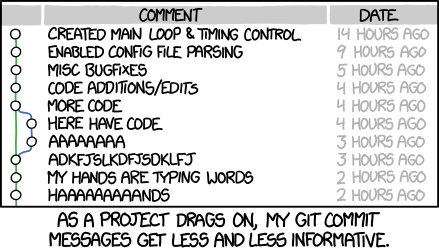
\includegraphics[width=.7\textwidth]{xkcd2.png}
\caption{\url{https://xkcd.com/1296/}}
\end{figure}


\subsection*{Index of Git Commands} % -----------------------------------------

\begin{table}[H]
\centering
\begin{tabular}{l|l}
Command & Description \\ \hline
\li{git pull origin master} & Pull down changes from the master copy (synchronize).\\
\li{git add <filename(s)>} & Add a file or files to the list of things to be synced.\\
\li{git commit -m <<\"<message>\">>} & Package up the changes and give them a label (checkpoint).\\
\li{git push origin master} & Push committed changes up to the master copy\\
\li{git status} & See which files have been changed and which have been\\&added to the commit.\\
\li{git diff <filename>} & See the changes made on a particular file since the\\&latest commit.\\
\li{git checkout -- <filename>} & Revoke the changes made since the last commit.\\
\li{git log} & See the commit history.\\
\li{git revert} & Revert to the state of the last commit.
\end{tabular}
\end{table}

\begin{figure}
\centering
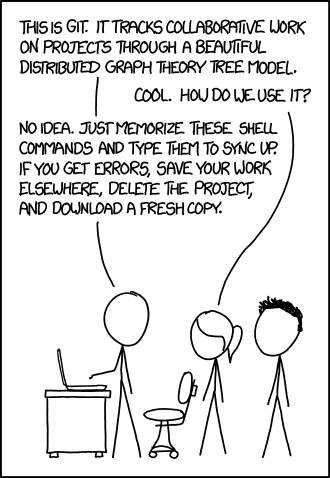
\includegraphics[width=\textwidth]{xkcd1.png}
\caption{\url{https://xkcd.com/1597/}}
\end{figure}

\section*{Lab Submission and File Organization} % =============================

Since the repositories for each class are entirely separate, we will use the convention \texttt{repository/lab\#/solutions.py}.
As long as we set up the repositories correctly online, the repository folder on your machine can be called whatever you want.

Git is designed to store source code files, not large data files.
When a lab uses a large data set, download the data and put it in your repository folder, but do not add or commit the data file.
That way, you can use the data locally without pushing it up to the cloud.

Please do not submit \emph{anything} other than the source code needed to run your solutions.
In addition, no file you submit should ever execute any code in its main body.
The only things you should include in the main body of the file are import statements, function declarations, and class declarations.
Anything else (tests, etc.) should be placed in an \li{if __name__ == "__main__":} block at the end of the file so that it is not executed when we import the file for grading.

